\documentclass[border=12pt, varwidth=38cm]{standalone}
\usepackage{tikz}
\usetikzlibrary{arrows.meta,positioning,calc,fit,backgrounds}
\usepackage{times}

\begin{document}
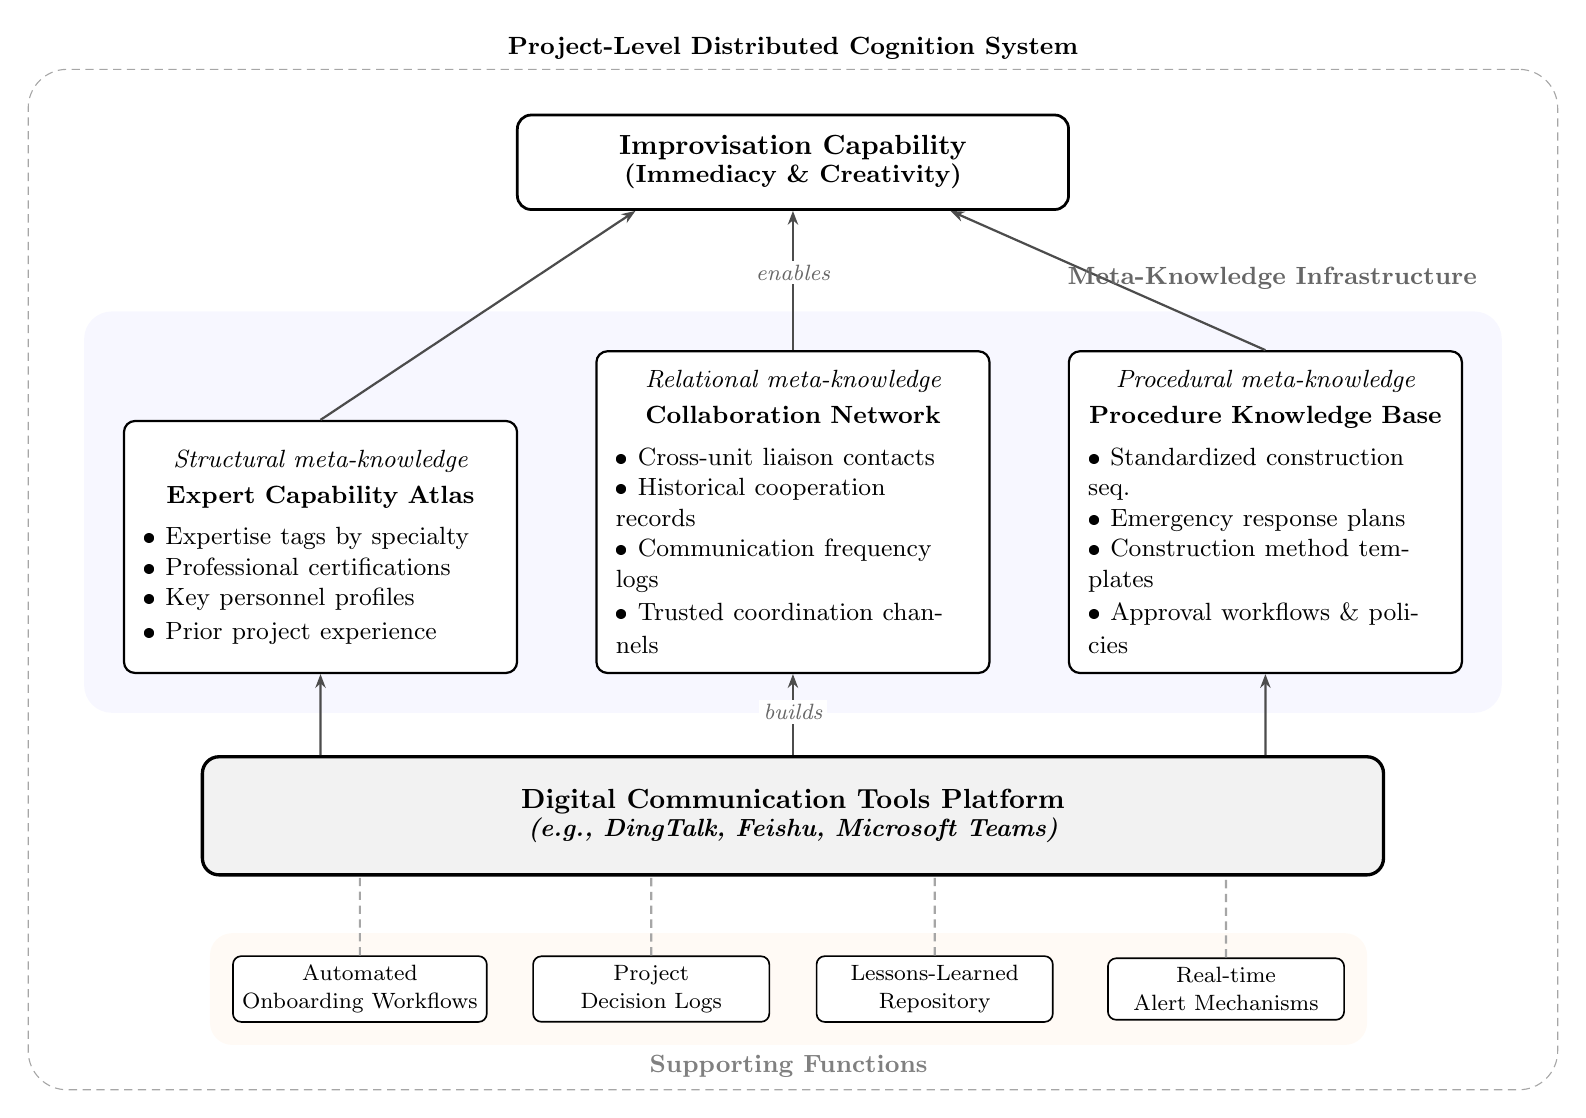
\begin{tikzpicture}[
  % === Node styles ===
  hub/.style={
    draw, rounded corners=6pt,
    minimum width=15cm, minimum height=1.5cm,
    font=\normalsize\bfseries, fill=gray!10,
    align=center, line width=1.2pt
  },
  module/.style={
    draw, rounded corners=4pt,
    text width=4.5cm, align=left,
    fill=white, line width=0.8pt,
    inner sep=7pt, minimum height=3.2cm
  },
  support/.style={
    draw, rounded corners=3pt,
    minimum width=3cm, minimum height=0.75cm,
    font=\fontsize{8}{10}\selectfont, fill=white, align=center,
    line width=0.6pt
  },
  outcome/.style={
    draw, rounded corners=5pt,
    minimum width=7cm, minimum height=1.2cm,
    font=\normalsize\bfseries, fill=white,
    align=center, line width=1pt
  },
  % === Arrow styles ===
  arr/.style={-{Stealth[length=5pt]}, thick, black!70},
  conn/.style={thick, black!35, densely dashed},
  % === Label styles ===
  arrlbl/.style={font=\fontsize{8}{10}\selectfont\itshape, fill=white, inner sep=1.5pt, text=black!60},
]

% =============================================
% Layer 0: DCTs Platform (Central Hub)
% =============================================
\node[hub] (dct) at (0, 0) {
  Digital Communication Tools Platform\\[-2pt]
  {\small\itshape (e.g., DingTalk, Feishu, Microsoft Teams)}
};

% =============================================
% Layer 1: Three Meta-Knowledge Modules
% =============================================
\node[module, anchor=south] (sm) at (-6, 1.8) {
  {\centering\fontsize{9}{11}\selectfont\itshape Structural meta-knowledge\par}
  \vspace{2pt}
  {\centering\small\bfseries Expert Capability Atlas\par}
  \vspace{4pt}
  \fontsize{9}{11}\selectfont
  \textbullet~Expertise tags by specialty\\
  \textbullet~Professional certifications\\
  \textbullet~Key personnel profiles\\
  \textbullet~Prior project experience
};

\node[module, anchor=south] (rm) at (0, 1.8) {
  {\centering\fontsize{9}{11}\selectfont\itshape Relational meta-knowledge\par}
  \vspace{2pt}
  {\centering\small\bfseries Collaboration Network\par}
  \vspace{4pt}
  \fontsize{9}{11}\selectfont
  \textbullet~Cross-unit liaison contacts\\
  \textbullet~Historical cooperation records\\
  \textbullet~Communication frequency logs\\
  \textbullet~Trusted coordination channels
};

\node[module, anchor=south] (pm) at (6, 1.8) {
  {\centering\fontsize{9}{11}\selectfont\itshape Procedural meta-knowledge\par}
  \vspace{2pt}
  {\centering\small\bfseries Procedure Knowledge Base\par}
  \vspace{4pt}
  \fontsize{9}{11}\selectfont
  \textbullet~Standardized construction seq.\\
  \textbullet~Emergency response plans\\
  \textbullet~Construction method templates\\
  \textbullet~Approval workflows \& policies
};

% =============================================
% Layer 2: Improvisation Capability (Outcome)
% =============================================
\node[outcome] (ic) at (0, 8.3) {
  Improvisation Capability\\[-2pt]
  {\small (Immediacy \& Creativity)}
};

% =============================================
% Layer -1: Supporting Functions
% =============================================
\node[support] (s1) at (-5.5, -2.2) {Automated\\Onboarding Workflows};
\node[support] (s2) at (-1.8, -2.2) {Project\\Decision Logs};
\node[support] (s3) at (1.8, -2.2) {Lessons-Learned\\Repository};
\node[support] (s4) at (5.5, -2.2) {Real-time\\Alert Mechanisms};

% =============================================
% Arrows: DCTs → MK Modules
% =============================================
\draw[arr] ([xshift=-6cm]dct.north) -- (sm.south);
\draw[arr] (dct.north) -- (rm.south);
\draw[arr] ([xshift=6cm]dct.north) -- (pm.south);

% Arrow label (centered between DCTs and MK)
\node[arrlbl] at ([yshift=0.55cm]dct.north) {builds};

% =============================================
% Arrows: MK Modules → IC (unified)
% =============================================
\draw[arr] (sm.north) -- ([xshift=-2.0cm]ic.south);
\draw[arr] (rm.north) -- (ic.south);
\draw[arr] (pm.north) -- ([xshift=2.0cm]ic.south);

% Arrow label (centered between MK and IC)
\node[arrlbl] at (0, 6.9) {enables};

% =============================================
% Connections: Supporting Functions ↔ DCTs
% =============================================
\draw[conn] (s1.north) -- ([xshift=-5.5cm]dct.south);
\draw[conn] (s2.north) -- ([xshift=-1.8cm]dct.south);
\draw[conn] (s3.north) -- ([xshift=1.8cm]dct.south);
\draw[conn] (s4.north) -- ([xshift=5.5cm]dct.south);

% =============================================
% Background groupings
% =============================================
\begin{pgfonlayer}{background}
  % Meta-knowledge infrastructure group
  \node[fill=blue!3, rounded corners=10pt, inner xsep=14pt, inner ysep=14pt,
        fit=(sm)(rm)(pm)]
        (mkbg) {};
  % Supporting functions group
  \node[fill=orange!4, rounded corners=8pt, inner sep=8pt,
        fit=(s1)(s2)(s3)(s4),
        label={[font=\fontsize{9}{11}\selectfont\bfseries, text=black!50]below:Supporting Functions}]
        (supbg) {};
\end{pgfonlayer}

% MK group label (just above the top-right corner of the blue background box)
\node[font=\small\bfseries, text=black!60, anchor=south east] at ([yshift=0.15cm, xshift=-0.2cm]mkbg.north east) {Meta-Knowledge Infrastructure};

% =============================================
% Overall system frame
% =============================================
\node[draw=black!35, densely dashed, rounded corners=14pt,
      inner xsep=20pt, inner ysep=16pt,
      fit=(ic)(mkbg)(dct)(supbg),
      label={[font=\small\bfseries, anchor=south]above:Project-Level Distributed Cognition System}]
      {};

\end{tikzpicture}
\end{document}
